\documentclass[aspectratio=43,10pt]{beamer}
\usepackage[utf8]{inputenc}
\usepackage{amsmath}
\usepackage{amsfonts}
\usepackage{amssymb}
\usepackage{bbold}
\usepackage{graphicx,fancybox}
\usepackage{babel}
\usepackage{minted}
\usepackage{wrapfig}
\usepackage{verbatim}
\usepackage{appendixnumberbeamer}
\usepackage{physics}
\usepackage{multicol}
\usepackage{hyperref}
\hypersetup{
	colorlinks=true,
	linkcolor=blue,
	filecolor=magenta,
	urlcolor=blue,
}

\setlength{\columnseprule}{.5pt}
\def\columnseprulecolor{\color{black}}

% \graphicspath{{Notes/Images}}

\setbeamertemplate{footline}[frame number]
\beamertemplatenavigationsymbolsempty
\usetheme{Warsaw}
% \usetheme{Madrid}
% \usetheme{CambridgeUS}

\addtobeamertemplate{footline}{\hypersetup{allcolors=.}}{}
% \definecolor{uprmgreen}{RGB}{51, 113, 55}
\definecolor{crimsonflame}{RGB}{158, 27, 50}
\usecolortheme[named=crimsonflame]{structure}

\usefonttheme{professionalfonts}
% \usepackage{mathpazo}
\usepackage{mathptmx}
% \renewcommand\familydefault{\rmdefault}


\title[Lecture Notes]{PH - 541\\ Quantum Mechanics \\Lecture Notes}

% Updated on
\date[\today]{Updated on \today}

\author[G. Fidalgo]{Guillermo A. Fidalgo Rodríguez}
\institute[UA]{University of Alabama}
% \logo{\includegraphics[width = 1in]{uprm_logo.png}}
% \logo{
\includegraphics[width = 1cm]{Images/UA_logo.jpg}}


%%%%%%%%%%%%%%%%%%%%%%
% For adding TOC at every section
% \AtBeginSection[]
% {
%     \begin{frame}
%         \frametitle{Table of Contents}
%         \tableofcontents[currentsection]
%     \end{frame}
% }
% \AtBeginSubsection[]
% {
%     \begin{frame}
%         \frametitle{Table of Contents}
%         \tableofcontents[currentsubsection]
%     \end{frame}
% }
%%%%%%%%%%%%%%%%%%%%%

% For adding a slide at each section
% \AtBeginSubsection{
% \begin{frame}
% 	\vfill
% 	\centering
% 	% \begin{beamercolorbox}[sep=6pt,center,shadow=true,rounded=true]{title}
% 	  \usebeamerfont{title}
% 	  \insertsectionhead
% 	  \\ (\insertsubsectionhead)\par%
% 	% \end{beamercolorbox}
% 	\vfill
% \end{frame}
% }

\begin{document}
\begin{frame}
	\titlepage
	\hfill
	
\includegraphics[width=1.5cm]{Images/UA_logo.jpg}
\end{frame}

\begin{frame}{TOC}
	\tableofcontents
\end{frame}

\section{Base Kets and Matrix Representations}
\begin{frame}{Eigenkets of an observation}
	\begin{alertblock}{Theorem 1}
		The eigenvalues of a Hermitian operator $A$ are real; the eigenkets of $A$ corresponding to different eigenvalues are orthogonal.
	\end{alertblock}
	Proof:

	\begin{gather}
		A\ket{a'} = a'\ket{a'} \label{eq:1}\\
		\bra{a'' }A = a''^* \bra{a''} \label{eq:2}\\
		\bra{a''} \cdot \ref{eq:1} - \ref{eq:2}\cdot \ket{a'} \to (a'-a'') \ip{a''}{a'} = 0
	\end{gather}
	If $a'=a''$, then $a'=a''^*=a'^*$ since $\ip{a'}{a'} = 0$

	$\therefore a'$ is real. If $a'\ne a'', a'-a'' \ne 0 \Longrightarrow \ip{a''}{a'} = 0$

	i.e. $\ket{a''} \& \ket{a'}$ are orthogonal.

\end{frame}
\begin{frame}
	Can normalize $\ket{a'}$ so that $\{\ket{a'}\}$ forms an orthogonal set with $\ip{a''}{a'}= \delta_{a' a''}$.

	The set of eigenkets forms a complete set to span the ket space.
\end{frame}

\subsection{Eigenkets and Base Kets}
\begin{frame}
	\frametitle{Eigenkets and Base Kets}

	\begin{equation}\label{eq:alpha base}
		\ket{\alpha} = \sum_{a'} C_{a'} \ket{a'}
	\end{equation}
	--- expansion of an arbitrary ket in the ket space spanned by the eigenkets of $A$.
	\begin{gather*}
		\bra{a''} (\ref{eq:alpha base}): \quad \ip{a''}{\alpha} = \sum_{a'} C_{a'} \underbrace{\ip{a''}{a'}}_{\delta_{a'' a'}} = C_{a''}\\
		\Rightarrow C_{a'} = \ip{a'}{\alpha}\\
		\therefore \quad \ket{\alpha} = \sum_{a'} \op{a'}\ket{\alpha}\\
		\text{C.f.} \quad \vec{V} = \sum_i \hat e_i (\hat e_i \cdot \vec V) \qq{for a vector} \vec V
	\end{gather*}
\end{frame}


\begin{frame}
	\frametitle{Completeness relation or closure relation}
	$$
		\mathbb{1} = \sum_{a'} \op{a'}
	$$
	eg.
	\begin{columns}
		\column{.5\textwidth}
		\begin{gather*}
			\ip{\alpha} = \bra{\alpha} \cdot \qty(\sum_{a'}\op{a'}) \cdot \ket{\alpha}	\\
			= \sum_{a'} \ip{\alpha}{a'}\ip{a'}{\alpha}\\
			= \sum_{a'} \ip{a'}{\alpha}^*\ip{a'}{\alpha}\\
			= \sum_{a'} \qty|\ip{a'}{\alpha}|^2
		\end{gather*}
		\column{.5\textwidth}
		also if $\ket{\alpha}$ is normalized then $\ip{\alpha}  = 1$
		\begin{align*}
			\Rightarrow & \sum_{a'} \qty|\ip{a'}{\alpha}|^2 \\
			            & = \sum_{a'} |C_{a'}|^2            \\
			            & = 1
		\end{align*}
	\end{columns}
\end{frame}
\begin{frame}
	\frametitle{Projection operator}

	Note: $\op{a'}$ is a projection operator because
	\[
		\qty(\op{a'})\cdot \ket{\alpha} = \ket{a'} \ip{a'}{\alpha} = C_{a'} \ket{a'}
	\]
	c.f. Dyadic ooperator in 3D Euclidean space
	\[\hat e_i \hat e_j \qquad (\hat x \hat x) \cdot \bar V = \hat x (\hat x \cdot \bar V)\]
\end{frame}
\subsection{Matrix Representations}
\begin{frame}
	\frametitle{Matrix Representations}
	A ket can be represented as a column vector.\\
	An operator can be represented as a matrix.
	\[
		\ket \alpha = \sum_{a'} \ket{a'} \ip{a'}{\alpha}
	\]
	where $a'$ is a base ket.

	If we use a column vector to represent $\ket{a'}$ it will be the following. Denote
	\begin{gather*}
		\qty{a'} = \qty{a^{(1)},a^{(2)},\dots}\\
		\ket{a^{(1)}} = \mqty[1 \\ 0 \\ 0 \\ \vdots] \quad \ket{a^{(2)}} = \mqty[0 \\ 1 \\ 0 \\ \vdots]
	\end{gather*}

\end{frame}
\begin{frame}
	\frametitle{Matrix Representations}

	So
	\[
		\ket{\alpha} = \ket{a^{(1)}} = \mqty[\ip{a^{(1)}}{\alpha} \\ \ip{a^{(2)}}{\alpha} \\ \vdots] = \mqty[C_{a^{(1)}}\\C_{a^{(2)}}\\ \vdots]
	\]
	Operator $X$ in matrix form
	\[
		X = \mathbb{1} \cdot X \cdot \mathbb{1} = \sum_{a'} \op{a''} X\sum_{a'} \op{a'}  = \sum_{a'' a'} \op{a''} X \op{a'}
	\]
	\[
		X = \mqty[
			\ev{X}{a^{(1)}} & \mel{a^{(1)}}{X}{a^{(2)}} & \cdots \\
			\mel{a^{(2)}}{X}{a^{(1)}} & \ev{X}{a^{(2)}} & \cdots \\
			\vdots & \vdots & \ddots
		]
	\]
	is a square matrix
	Note:

	\[
		\mel{a'' }{X}{a'} = \mel{a'}{X^\dag}{a''}^* \Rightarrow \mel{a'}{X^\dag}{a''} = \mel{a''}{X}{a'}^*
	\]
	Hermitian adjoint corresponds to taking the transpose and complex conjugate of the matrix form of the operator.
\end{frame}

\begin{frame}
	\frametitle{Matrix Representations}

	\begin{gather*}
		Z = XY\\
		\mel{a''}{Z}{a'} = \mel{a''}{XY}{a'} \\
		= \sum_{a'''} \mel{a''}{X}{a'''} \mel{a'''}{Y}{a'}\\
		\ket{\gamma} = X \ket{\alpha}\\
		\ip{a'}{\gamma} = \mel{a'}{X}{\alpha} \Rightarrow \sum_{a''} \mel{a'}{X}{a''}\ip{a''}{\alpha} \\
		\mqty[\ip{a^{(1)}}{\gamma} \\ \ip{a^{(2)}}{\gamma} \\ \vdots] = \mqty[
			\ev{X}{a^{(1)}} & \mel{a^{(1)}}{X}{a^{(2)}} & \cdots \\
			\mel{a^{(2)}}{X}{a^{(1)}} & \ev{X}{a^{(2)}} & \cdots \\
			\vdots & \vdots & \ddots
		] \mqty[\ip{a^{(1)}}{\alpha} \\ \ip{a^{(2)}}{\alpha} \\ \vdots]
	\end{gather*}
	same for bras
\end{frame}

\begin{frame}{Matrix Representations}
	\begin{gather*}
		\bra{\gamma} = \bra{\alpha} X \\
		\ip{\gamma}{a'} = \mel{\alpha}{X}{a'} = \sum_{a''} \ip{\alpha}{a''}\mel{a'' }{X}{a'}\\
		= \mqty[\ip{\gamma}{a^{(1)}} & \ip{\gamma}{a^{(2)}} & \cdots]  \\
		= \mqty[\ip{\alpha}{a^{(1)}} & \ip{\alpha}{a^{(2)}} & \cdots]
		\mqty[
			\ev{X}{a^{(1)}} & \mel{a^{(1)}}{X}{a^{(2)}} & \cdots \\
			\mel{a^{(2)}}{X}{a^{(1)}} & \ev{X}{a^{(2)}} & \cdots \\
			\vdots & \vdots & \ddots
		]
	\end{gather*}

\end{frame}

\begin{frame}{Matrix Representations}
	For inner products
	\begin{gather*}
		\ip{\beta}{\alpha} = \sum_{a'} \ip{\beta}{a'}\ip{a'}{\alpha} \\
		= \mqty[ \ip{\beta}{a^{(1)}} & \ip{\beta}{a^{(2)}} & \cdots]
		\mqty[ \ip{a^{(1)}}{\alpha} \\
			\ip{a^{(2)}}{\alpha} \\
			\vdots]
		\\
	\end{gather*}
	For outer products
	\begin{gather*}
		\op{\beta}{\alpha} = \qty(\sum_{a''} \op{a''}) \ket\beta \bra{\alpha} \qty(\sum_{a'} \op{a'})=\sum_{a' a''} \op{a''}\op{\beta}{\alpha} \op{a'} \\
		= \ip{a'''}{\beta} \ip{\alpha}{a'''} = \mqty[
			\ip{a^{(1)}}{\beta}\ip{a^{(1)}}{\alpha}^* & \ip{a^{(1)}}{\beta}\ip{a^{(2)}}{\alpha}^* & \cdots \\
			\ip{a^{(2)}}{\beta}\ip{a^{(1)}}{\alpha}^* & \ip{a^{(2)}}{\beta}\ip{a^{(1)}}{\alpha}^* & \cdots \\
			\vdots & \vdots & \ddots
		]
	\end{gather*}
\end{frame}

\begin{frame}{Matrix Representations}
	\begin{itemize}
		\item If $\{\ket{a'}\}$ is the set of eigenkets of the operator $A = \mathbb{1}\cdot A \cdot \mathbb{1}$
	\end{itemize}
	\begin{gather*}
		\sum_{a'' a'} \op{a''} \underbrace{A\ket{a'}}_{a'\ket{a'}}\bra{a'} = \sum_{a' a''} a'\ket{a'}\underbrace{\ip{a''}{a'}}_{\delta_{a'' a'}} \ket{a'} = \sum_{a'} a'\op{a'}\\
		\mqty[\dmat{ a^{(1)},a^{(2)},\ddots }]
	\end{gather*}
\end{frame}

\begin{frame}{Example: Spin 1/2 systems}
	Base kets : $ \ket{S_z;\pm} = \ket{\pm}$\\
	Completeness: $\mathbb{1} = \op{+} + \op{-}$
	\begin{gather*}
		\text{Eigenvalue eqn}: S_z \ket{\pm} = \pm \frac\hbar2 \ket{\pm}\\
		S_z = \frac\hbar2 \op{+} - \frac{\hbar}{2}\op{-} = \frac{\hbar}{2} \qty(\op{+} - \op{-})
	\end{gather*}
\end{frame}

\subsection{Example: Spin 1/2 systems}
\begin{frame}{Example: Spin 1/2 systems}

	Now define

	\[
		\begin{split}
			S_+ = \hbar \op{+}{-} \\
			S_- = \hbar \op{-}{+}
		\end{split}\Biggr\} \text{Ladder Operators}
	\]

	Note:
	\[
		\begin{split}
			S_+ \ket{-} = \hbar \ket + \overbrace{\ip{-}}^1 = \hbar\ket + \\
			S_+ \ket{+} = \hbar \ket + \underbrace{\ip{-}{+}}_0 =  0      \\
		\end{split} \Biggr\} \text{Raising Operator}
	\]
	%
	\[
		\begin{split}
			S_- \ket{+} = \hbar \ket - \overbrace{\ip{+}}^1 = \hbar\ket - \\
			S_- \ket{-} = \hbar \ket - \underbrace{\ip{+}{-}}_0 =  0      \\
		\end{split} \Biggr\} \text{Lowering Operator}
	\]

\end{frame}


\begin{frame}{Matrix Representations}{Spin 1/2 systems}
	$$\ket{+} = \mqty[1 \\ 0] \qquad \ket- = \mqty[0 \\ 1]$$
	\begin{gather*}
		S_z \doteq \frac{\hbar}{2} \pqty{\mqty[1\\0] \mqty[1 & 0] - \mqty[0 \\ 1] \mqty[0 & 1]} = \frac{\hbar}{2} \mqty[\pmat{3}]\\
		S_+ = \hbar \op{+}{-} = \hbar \mqty[1 \\ 0 ] \mqty[0 & 1] = \hbar \mqty[0 & 1\\0 & 0]\\
		S_- = \hbar \mqty[0&0\\1&0]
	\end{gather*}
\end{frame}


\section{Measurements, Observables and the Uncertainty Relations}
\begin{frame}{Measurements, Observables and the Uncertainty Relations}{Measurements}
	\begin{itemize}
		\item Observable A \\
		      Before measurement, the system is in a state $\ket \alpha$
		      \[
			      \ket{\alpha} = \sum_{a'} \ket{a'} \ip{a'}{\alpha}
		      \]
		      where $\{\ket{a'}\}$ is the set of eigenkets for $A$. Under measuerment the system is thrown into an eigenstate
		      \[ \ket{\alpha} \xrightarrow{\text{ \tiny A measurement}} \ket{a'}\]
		      If the state before measurement is an eigenstate of the observables, say $\ket{a'}$
		      \[ \ket{a'} \xrightarrow{\text{\tiny A measurement}} \ket{a'}\]
	\end{itemize}
\end{frame}

\begin{frame}
	\begin{itemize}
		\item Probability for jumping into some particular state $\ket{a'}$ is $|\ip{a'}{\alpha}|^2$ where $\ket{\alpha}$ is normalized.
		      In the particular case when $\ket{\alpha} = \ket{a'}$ before measurement, then probability of measuring $A$ to be $a'$ will be 1 since
		      \[\qty|\ip{a'}|^2 = 1\]
		      Probability of measuring $A$ to be $a''$ (where $a'' \neq a'$) will be 0 since $\qty|\ip{a''}{a'}|^2 = 0$ due to orthogonality.
		\item Expectation value of $A$ when the system is in state $\ket \alpha$. \[\ev{A} =\ev{A}{\alpha} \]
		      means the average measured value
		      \begin{gather*}
			      \ev{A} = \sum_{a''}\sum_{a'} \ip{\alpha}{a''}\mel{a''}{A}{a'}\ip{a'}{\alpha}\\
			      = \sum_{a''}\sum_{a'} a'\ip{\alpha}{a''} \underbrace{\ip{a''}{a'}}_{\delta_{a''a'}} \ip{a'}{\alpha}\\
			      = \sum_{a'} a' \ip{\alpha}{a'}\ip{a'}{\alpha} = \sum_{a'} a' \ip{a'}{\alpha} \ip{a'}{\alpha}^* = \sum_{a'} a'|\ip{a'}{\alpha}|^2
		      \end{gather*}
	\end{itemize}
\end{frame}

\subsection{Compatible Observables}
\begin{frame}{Compatible Observables}
	\begin{itemize}
		\item Compatible observables if $\comm{A}{B} = 0$, otherwise they are called incompatible. e.g.
		      \begin{gather*}
			      \comm{S^2}{S_z} = 0 \Rightarrow S^2,S_z \; \text{are compatible}\\
			      \comm{S_x}{S_z} \neq 0 \Rightarrow S_x,S_z \; \text{are incompatible}
		      \end{gather*}
		\item Suppose there are two (or more) linearly independent eigenkets of $A$ having the same eigenvalue, then the eigenvalues of the two eigenkets are said to be degenerate. e.g. $\left\{ a^{(1)}, a^{(2)},\dots,a^{(k)}\right\}$ correspond to $\left\{\ket{a^{(1)}},\ket{a^{(2)}},\dots,\ket{a^{(k)}}	\right\}$
		      If $a^{(1)} = a^{(2)} = a, \ket{a^{(1)}} \& \ket{a^{(2)}}$ are degenerate states $\Rightarrow \{a,a,a^{(3)} ,\dots\}$. How to distinguish them?
	\end{itemize}
\end{frame}

\begin{frame}{Compatible Observables}
	\begin{alertblock}{Theorem 2}
		Suppose $A \ \&\  B$ are compatible observables, and the eigenvalues of $A$ are non-degenerate. Then, the matrix elements $\mel{a''}{B}{a'}$ are all diagonal.
	\end{alertblock}

	Proof:
	\begin{align*}
		\mel{a''}{\comm{A}{B}}{a'} & = \mel{a''}{(AB - BA)}{a'}    \\
		                           & = \mel{a''}{(a''B -B a')}{a'} \\
		                           & = (a'' - a') \mel{a''}{B}{a'} \\
		                           & = 0
	\end{align*}
	$\mel{a''}{B}{a'} = 0 $ unless $a'' = a'$
	\[
		\mqty[\ddots\admat{0,\ddots,0}\ddots]
	\]
\end{frame}

\begin{frame}
	If $\comm{A}{B} = 0$ and eigenvalues of $A$ are non-degenerate $ \mel{a''}{B}{a'} $ are diagonal.
	\begin{gather*}
		\mel{a''}{B}{a'}  = \delta_{a'a''} \ev{B}{a'}\\
		B = \mathbb{1}\cdot B \cdot \mathbb{1} = \sum_{a' a''} \ket{a''} \underbrace{\mel{a''}{B}{a'} }_{\delta_{a'a'} \ev{B}{a'}}\bra{a'}\\
		\sum_{a''}\ket{a''}\mel{a''}{B}{a''} \bra{a''}\\
		B\ket{a'} = \sum_{a''} \ket{a''}\mel{a''}{B}{a''}\underbrace{\ip{a''}{a'}}_{\delta_{a'a''}}\\
		= \ket{a'} \underbrace{\mel{a'}{B}{a'}}_{b'} = b'\ket{a'} \; \to \text{eigenvalue eq. for }B.
	\end{gather*}
	$\ket{a'}$ is a simultaneous eigenket of $A$ and $B$ labeled as $\ket{a',b'}$
	\begin{align*}
		A\ket{a',b'} & =a'\ket{a',b'} \\
		B\ket{a',b'} & =b'\ket{a',b'}
	\end{align*}
\end{frame}

\begin{frame}
	If we have a maximal set of mutually commuting observables $A,B,\dots$ with $\comm{A}{B}=\comm{B}{C}=\comm{A}{C}= 0$.\\
	Simultaneous eigenkets are labeled as $\ket{k'} = \ket{a',b',c',\dots}$.
	\begin{itemize}
		\item Orthonormality: $\ip{k''}{k'} = \delta_{k''k'}=\delta_{a''a'}\delta_{b''b'}\delta_{c''c'}$
		\item Completeness: $\sum_{k'}\op{k'} = \sum_a' \sum_b' \sum_c' \dots \op{a',b',c',\dots} = \mathbb{1}$
	\end{itemize}
\end{frame}

\begin{frame}{What happens if we measure two compatible observables $A$ and $B$?}
	\begin{itemize}
		\item If eigenvalues of $A$ are non-degenerate:
		      \[
			      \ket{\alpha} \xrightarrow[A \text{ get } a']{\text{measurement}} \ket{a',b'} \xrightarrow[B \text{ get } b']{\text{measurement}} \ket{a',b'}\xrightarrow[A \text{ get } a']{\text{measurement}}\ket{a',b'}
		      \]
		\item If eigenvalues of $A$ are n-fold degenerate:
		      \[\tiny \hspace{-4mm}
			      \ket{\alpha} \xrightarrow[A \text{ get } a']{\text{measurement}} \sum_{i=1}^n C_{a}^{i}\ket{a',b^{(i)}} \xrightarrow[B \text{ get } b^{(j)}]{\text{measurement}} \ket{a',b^{(j)}}\xrightarrow[A \text{ get } a']{\text{measurement}}\ket{a',b^{(j)}}
		      \]
	\end{itemize}

	$A$ measurements and $B$ measurements do not interfere for compatible observables.

	Note: Incompatible observables do not have a complete set of simultaneous eigenkets.
\end{frame}

% \item \textbf{Problem 1.6}  Using the rules of bra-ket algebra, prove or evaluate the following:
\begin{enumerate}
	\item $\Tr(XY) = \Tr(YX)$, where $X$ and $Y$ are operators.

	      \textbf{Solution:}
	      \begin{gather*}
		      \Tr(XY) = \sum_{a'} \ev{XY}{a'} = \sum_{b'}\sum_{a'} \mel{a'}{X}{b'} \mel{b'}{Y}{a'} \\
		      = \sum_{b'a'} \mel{b'}{Y}{a'} \mel{a'}{X}{b'} = \sum_{b'} \mel{b'}{YX}{b'} = \Tr(YX)
	      \end{gather*}

	\item $(XY)^\dag = Y^\dagger X^\dag$, where $X$ and $Y$ are operators.

	      \textbf{Solution:}

	      Using two arbitrary kets $\ket \alpha, \ket \beta$
	      \begin{gather*}
		      \mel{\alpha}{(XY)^\dag}{\beta} = \mel{\beta}{XY}{\alpha}^* = \sum_{a'} \qty(\mel{\beta}{X}{a'}\mel{a'}{Y}{\alpha})^* = \sum_{a'} \mel{a'}{Y}{\alpha}^* \mel{\beta}{X}{a'}^* \\
		      = \sum_{a'}\mel{\alpha}{Y^\dag}{a'}\mel{a'}{X^\dag}{\beta} = \mel{\alpha}{Y^\dag X^\dag}{\beta}
	      \end{gather*}
	      So we have

	      \[
		      \mel{\alpha}{(XY)^\dag}{\beta}=\mel{\alpha}{Y^\dag X^\dag}{\beta}
	      \]
	      for arbitrary $\ket \alpha, \ket \beta$, therefore we must have
	      \[
		      (XY)^\dag = Y^\dagger X^\dag
	      \]



	\item $\exp[if(A)] =?$ in ket-bra form, where A is a Hermitian operator whose eigenvalues are known.

	      \textbf{Solution:}

	      \begin{gather*}
		      \exp[if(A)] = \exp[if\qty(\sum_{a'a''} \op{a'} A \op{a''})] \\
		      = \exp(if \mqty[\dmat[0]{a',a'' , \ddots}]) = \mqty[\dmat[0]{\exp(if(a')),\exp(if(a'')), \ddots}]\\
		      = \sum_{a'}\exp[if(a')]\op{a'}
	      \end{gather*}



\end{enumerate}

%\item \textbf{Problem 1.7}
\begin{enumerate}
    \item Consider two kets $\ket \alpha$ and $\ket \beta$. Suppose $\ip{a'}{\alpha}, \ip{a''}{\alpha}, \dots$and $\ip{a'}{\beta}, \ip{a''}{\beta}, \dots$ are all known, where $\ket{a'}, \ket{a''}, \dots$ form a complete set of base kets. Find the matrix representation of the operator $\op{\alpha}{\beta}$.

    \begin{gather*}
        \ket \alpha = \sum_{a'} \ket{a'}\ip{a'}{\alpha}\\
        \ket \beta = \sum_{a''} \ket{a''}\ip{a''}{\beta}
    \end{gather*}

    Now we evaluate $\op{\alpha}{\beta}$ and set $\op{\alpha}{\beta} = Z$
    \begin{gather*}
        \sum_{a'' a'} \ket{a'}\ip{a'}{\alpha} \ip{\beta}{a''}\bra{a'' }  = \sum_{a'a''} \op{a'}Z \op{a''}\\
        \mqty(\mel{a^1}{Z}{a^1} & \mel{a^1}{Z}{a^2} & \cdots & \mel{a^1}{Z}{a^m} \\
        \mel{a^2}{Z}{a^1} & \mel{a^2}{Z}{a^2} & \cdots & \mel{a^2}{Z}{a^m} \\
        \vdots & \vdots & \ddots & \vdots\\
        \mel{a^m}{Z}{a^1} & \cdots & \cdots & \mel{a^m}{Z}{a^m}
        )
    \end{gather*}



    \item We know consider a spin $\frac12$ system and let $\ket \alpha$ and $\ket \beta$ be $\ket{S_z;+}$ and $\ket{S_x;+}$, respectively. Write down explicitly the square matrix that corresponds to $\op{\alpha}{\beta}$ in the usual ($s_z$ diagonal) basis.

    \begin{gather*}
    \ket \alpha = \ket{S_z;+} = \ket + = \mqty(1 \\0 )\\
    \ket{\beta} = \ket{S_x;+} = \frac{1}{\sqrt2}(\ket + + \ket -) = \frac{1}{\sqrt{2} } \mqty(1 \\ 1) \\
    \op{\alpha}{\beta} = \frac{1}{\sqrt{2}}\mqty(1\\0)\mqty(1&1) = \frac{1}{\sqrt2}\mqty(1&1\\0&0)
    \end{gather*}


\end{enumerate}

%\item \textbf{Problem 1.11}
Construct $\ket{\vb S\cdot\vu n;+}$ such that
\[
\vb S \cdot \vu n \ket{\vb S\cdot\vu n;+} = \qty(\frac{\hbar}{2}) \ket{\vb S\cdot\vu n;+}
\]
where $\vu n$ is characterized by the angles shown in the figure. Express your answer as a
linear combination of $\ket+$ and $\ket -$. [Note: The answer is
\[
\cos(\frac \beta2) \ket + \sin(\frac \beta2) e^{i\alpha}\ket -.
\]
\begin{figure}[h]
    \centering
    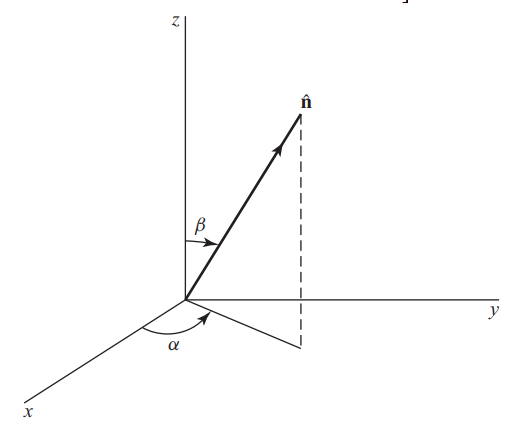
\includegraphics[width=0.5\linewidth]{P4.png}
\end{figure}

\textbf{Solution}

We begin by writing the matrix representation of this eigenvalue problem and then solving the eigenvalue problem stated above with the given eigenvalue $\frac{\hbar}{2}$ to find the eigenvector.

\begin{gather*}
\vb S \cdot \vu n = S_x \sin\beta \cos\alpha + S_y \sin\beta\sin\alpha + S_z \cos\beta\\
=\frac\hbar2 \mqty(\cos\beta & \sin\beta\cos\alpha - i\sin\beta\sin\alpha\\
                \sin\beta\cos\alpha + i\sin\beta\sin\alpha & -\cos\beta) = \frac\hbar2 \mqty(\cos\beta & \sin\beta e^{-i\alpha} \\ \sin\beta e^{i\alpha} & -\cos\beta)\\
\end{gather*}
We use this matrix and solve the eigenvalue equation
\begin{gather*}
    (\vb S\cdot \vu n - \frac\hbar2 \mathbb{I}) X = 0\\
    \frac{\hbar}{2} \mqty(\cos\beta -1 & \sin\beta e^{-i\alpha} \\ \sin\beta e^{i\alpha} & -\cos\beta - 1) \mqty(x \\ y) = \mqty(0\\0)\\
\end{gather*}
This gives us 2 equations

\begin{gather}
    (\cos\beta - 1)x + (\sin\beta e^{-i\alpha})y = 0\\
     (\sin\beta e^{i\alpha})x -(\cos\beta + 1)y = 0
\end{gather}
     From equation (2) we get the expression
     \[
     y= \frac{\sin\beta e^{i\alpha}}{\cos\beta+1} x
     \]

     And so our eigenvector can be written as
     \begin{gather*}
         \mqty[1 \\ \frac{\sin\beta e^{i\alpha}}{\cos\beta+1}] = \mqty[ 1 \\ \frac{\sin\beta e^{i\alpha}}{2\cos[2](\beta/2)}] = \mqty[\cos(\beta/2)\\ \frac{\sin\beta e^{i\alpha}}{2\cos(\beta/2)} ] = \mqty[  \cos\frac\beta2\\ \sin\frac\beta2 e^{i\alpha}  ]
     \end{gather*}

     Where I have used the relations
     \begin{align*}
         \cos\beta + 1 = 2\cos[2](\frac{\beta}{2}) && \sin\beta = 2\sin(\frac\beta2) \cos(\frac\beta2)
     \end{align*}
     and so using $x \to \ket +$ and $y \to \ket -$ we have

\[
\ket{\vb S\cdot\vu n;+} = \cos(\frac\beta2) \ket + + \sin(\frac\beta2)e^{i\alpha}
\]

%\include{Lecture_notes/P5}
% \include{Lecture_notes/P6}



\end{document}
